\chapter{Verification Dataset}
\label{chapter:vds}


\section{Overview}



\section{Correlative measurements}

\subsection{Aura/MLS}

The Aura satellite was launched on 2004-07-15 into a 
sun-synchronous orbit at 705\,km altitude, with an ascending
equator crossing local time of 13:45. Its
orbit is near-polar with a 98\degree inclination, 
and the daily Microwave Limb Sounder (MLS) measurements cover 
the latitudinal range from about 82\degree\,S to 82\degree\,N. 
MLS measures temperature and trace gas profiles 
using thermal emission data from the
upper troposphere to the mesosphere. MLS performs each
limb scan and related calibration in 25\,s, and 
obtains \(\sim\) 3500 vertical profiles a day 
\citep{waters2006}. The MLS data
processing algorithms are based on the optimal estimation
method (OEM), as explained by \citet{livesey2011}. MLS uses
spectral bands centered near 118, 190, 240, 640\,GHz,
and 2.3\,THz. 

\subsection{ENVISAT/MIPAS}

The Michelson Interferometer for Passive Atmospheric
Sounding (MIPAS) is a mid-infrared emission spectrometer
mounted on the European ENVIronmantal SATellite (ENVISAT),
which was launched in 2002-03-01 \citep{fischer2008}. 
ENVISAT has a sun-synchronous orbit at an altitude of 800\,km
and with a 98.55\degree inclination and descending equator 
crossing local time of 10:00.

MIPAS observed five mid-infrared spectral bands within the
frequency range of 685 to 2410\,cm\(^{-1}\) (14.6 to 4.15\,\(\mu\)m),
with a resolution of 0.0625\,cm\(^{-1}\).
Until 2004-03-26 MIPAS scanned 17 tangent altitudes from 
6 to 68\,km with 3,-\,8\,km resolution.
From January 2005 MIPAS started operating in a new mode
at a reduced spectral resolution but at a finer altitude
grid. The latitudinal coverage was from 87\degree\,S to 89\degree\,N.
In the latter mode, MIPAS had about 95 scans per orbit, and about
1360 vertical profiles were recorded in a day.

Opertaional Level-2 data from MIPAS is generated by ESA,
but we here consider the MIPAS scientific data product
generated by the Institut fur Meteorologie und Klimatforscung
(IMK) at Karlsruhe Institude of Technology (KIT).
This data product was retrieved using a Tikhonov-type
regularization with a smoothing constraint.


\subsection{ISS/JEM/SMILES}

The Superconducting Submillimeter-Wave Limb-Emission Sounder (SMILES),
attached to the Exposed Facility of the Japanese Experiment Module (JEM), 
on the International Space Station (ISS), is a joint project of the
National Institute of Information and Communications Technology (NICT) and
the Japan Aerospace Exploration Agency (JAXA).

SMILES, carried by ISS, collected thermal emission
between 2009-10-12 and 2010-04-21.
The ISS has a non-sun-synchronous circular orbit at
altitudes of 340\,-\,360\,km with an inclination angle of 51.6\degree
to the equator. The nominal latitude coverage of SMILES is from 38\degree\,S
to 65\degree\,N.

SMILES observed a number  
of trace gases, e.g.: \chem{O_{3}}, \chem{H^{35}Cl}, \chem{H^{37}Cl}, 
\chem{ClO}, \chem{HOCl}, \chem{HO_{2}}, \chem{BrO}, and \chem{HNO_{3}}, 
from the upper troposphere up to the lower thermosphere,  
between 2009-10-12 and 2010-04-21, and with a nominal latitudinal coverage 
from 38\degree\,S to 65\degree\,N.

SMILES collected atmospheric thermal emission in two frequency
bands around 625\,GHz and one around 650\,GHz;
624.32\,-\,625.52\,GHz (Band-A), 625.12\,-\,626.32\,GHz (Band-B),
and 649.12\,-\,650.32\,GHz (Band-C), with a frequency resolution
and channel separation of about 1\,MHz and 0.8\,MHz, 
respectively.  
During each measurement, two out of the three SMILES frequency
bands were observed simultaneously, by two acousto optical spectrometers,
and with a receiver noise temperature of 310\,-\,350\,K.

SMILES performed 1630 scans per day, where the limb was scanned
from about -20\,km to 120\,km (geometric altitude), 
with a sampling interval of about 2\,km, and with an angle of 
about 45\degree from the orbital plane. The size of the antenna beam, 
at the tangent point, was about 3 and 6\,km in the vertical and 
horizontal direction, respectively. 

An interesting feature of SMILES observation is related to the fact
that ISS has a non-sunsynchronous orbit, which gives that SMILES 
observations cover different local times and thereby provides insight
of the diurnal variation of atmospheric short-lived species
(e.g \chem{ClO}, \chem{BrO}, \chem{HO_2}, and \chem{HOCl}). 
A two month period is required to accumulate measurements covering 
24\,h in local time for a given "position". However, such a 
dataset can also contain variation due to dynamical, seasonal, and 
latitudinal effects.
A second characteristic of SMILES observation is that 
measured spectra and retrieved profiles have high precision due 
to its 4\,K mechanically cooled superconducting receiver system.



\subsection{Odin/OSIRIS}
 
text ...

\subsection{Meteor3M/SAGE III}
SAGE III on Meteor-3M (SAGE III/M3M) was a third generation, satellite-borne
instrument and an element in NASA’s Earth Observing System (EOS). The
instrument was launched on the Russian Meteor-3M spacecraft on 10 December 2001
into into a Sun-synchronous orbit at an altitude of 1020 km and with an
approximate 9:00 a.m. equatorial crossing time.  The instrument was active from
2002-02-27 to 2005-11-12.\footnote{all text in this section adapted from
\cite{SAGEIII_DPUG}}

The SAGE III instrument measures the attenuation of solar radiation resulting
from the scattering and absorption by atmospheric constituents in the Earth’s
atmosphere as the spacecraft observes a sunrise or sunset event.  Due to the
orbital parameters, solar occultation measurement opportunities are limited to
mostly high latitudes in the Northern Hemisphere (between 50\degree~and
80\degree~N) and mid-latitudes in the Southern Hemisphere (between
30\degree~and 50°~S).  Level~2 products from these measurements include
profiles of ozone~(\chem{O_3}), water vapour~(\chem{H_2O}) and nitrogen
dioxide~(\chem{NO_2}).  Of these \chem{O_3} and \chem{H_2O} have been included
in the VDS.  The ozone profiles are are reported as reliable within 10\% for
the altitude range 6--85\,km, whereas the water vapour profiles are reported
reliable to have an uncertainty of less than 5\% for altitudes of 0--33\,km and
in the interval 5--15\% for altitudes 33--50\,km.

Similar measurements where made during the lunar moonrise and moonset. Due to
poor data coverage, none of these products have been included in the VDS, but
are listed here for completeness.  These measurements were made only during the
second and third quarter phases of the Moon and when the atmosphere along the
line-of-sight was not directly illuminated by the Sun.  Level~2 products from
these measurements include profiles of ozone~(\chem{O_3}), nitrogen
dioxide~(\chem{NO_2}), nitrogen trioxide~(\chem{NO_3}) and chlorine
dioxide~(\chem{OClO}).



\section{Collocations criteria and scan selection}
 
text ...

\begin{table}
\caption{ \smr\ VDS content.}
\label{table:comp}
\begin{tabular}{|l|l|l|}
\hline
\textbf{Frequency mode} & \textbf{Instrument} &  \textbf{Species}\\
\hline
    1  &     SMILES   &      \chem{O_3} \\
       &     MLS      &      \chem{O_3}, \chem{ClO}, \chem{N_{2}O} \\
       &     MIPAS    &      \chem{O_3}, \chem{N_{2}O} \\
       &     SAGEIII  &      \chem{O_3} \\
\hline
    2  &     SMILES   &      \chem{O_3}, \chem{HNO_3} \\
       &     MLS      &      \chem{O_3}, \chem{HNO_3} \\
       &     MIPAS    &      \chem{O_3}, \chem{HNO_3} \\
       &     SAGEIII  &      \chem{O_3} \\
\hline
    8  &     SMILES   &      \chem{O_3} \\
       &     MLS      &      \chem{O_3}, \chem{H_{2}O} \\
       &     MIPAS    &      \chem{O_3}, \chem{H_{2}O} \\
       &     SAGEIII  &      \chem{O_3}, \chem{H_{2}O} \\
\hline
   13  &     SMILES   &      \chem{O_3} \\
       &     MLS      &      \chem{O_3}, \chem{H_{2}O} \\
       &     MIPAS    &      \chem{O_3}, \chem{H_{2}O} \\
       &     SAGEIII  &      \chem{O_3}, \chem{H_{2}O} \\
\hline
   17  &     SMILES   &      \chem{O_3} \\
       &     MLS      &      \chem{O_3}, \chem{H_{2}O} \\
       &     MIPAS    &      \chem{O_3}, \chem{H_{2}O} \\
       &     SAGEIII  &      \chem{O_3}, \chem{H_{2}O} \\
\hline
   19  &     SMILES   &      \chem{O_3} \\
       &     MLS      &      \chem{O_3}, \chem{H_{2}O} \\
       &     MIPAS    &      \chem{O_3}, \chem{H_{2}O} \\
       &     SAGEIII  &      \chem{O_3}, \chem{H_{2}O} \\
\hline
   21  &     SMILES   &      \chem{O_3}, \chem{NO} \\
       &     MLS      &      \chem{O_3}, \chem{H_{2}O} \\
       &     MIPAS    &      \chem{O_3}, \chem{H_{2}O} \\
       &     SAGEIII  &      \chem{O_3}, \chem{H_{2}O} \\
\hline
\end{tabular}
\end{table}


\clearpage
\newpage

\subsection{Frequency mode 1}

\begin{figure}[t]
\centering
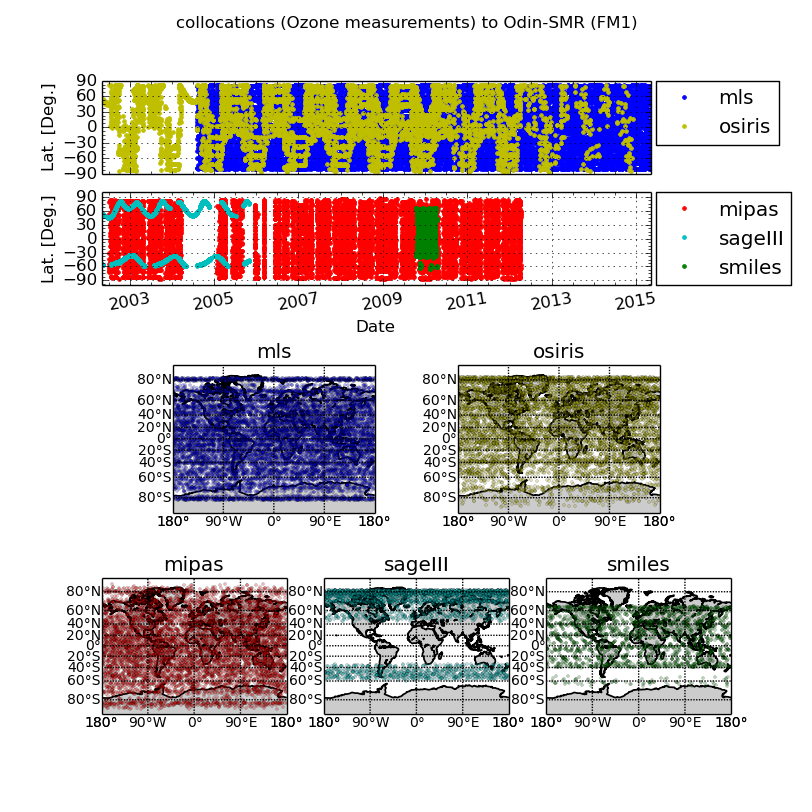
\includegraphics[width=17cm]{test_collocation_fm1.png}
\caption{VDS:Positions of collocated scans for frequency mode 1.}
\label{fig:vdsfm1}
\end{figure}


\clearpage
\newpage

\subsection{Frequency mode 2}

\begin{figure}[t]
\centering
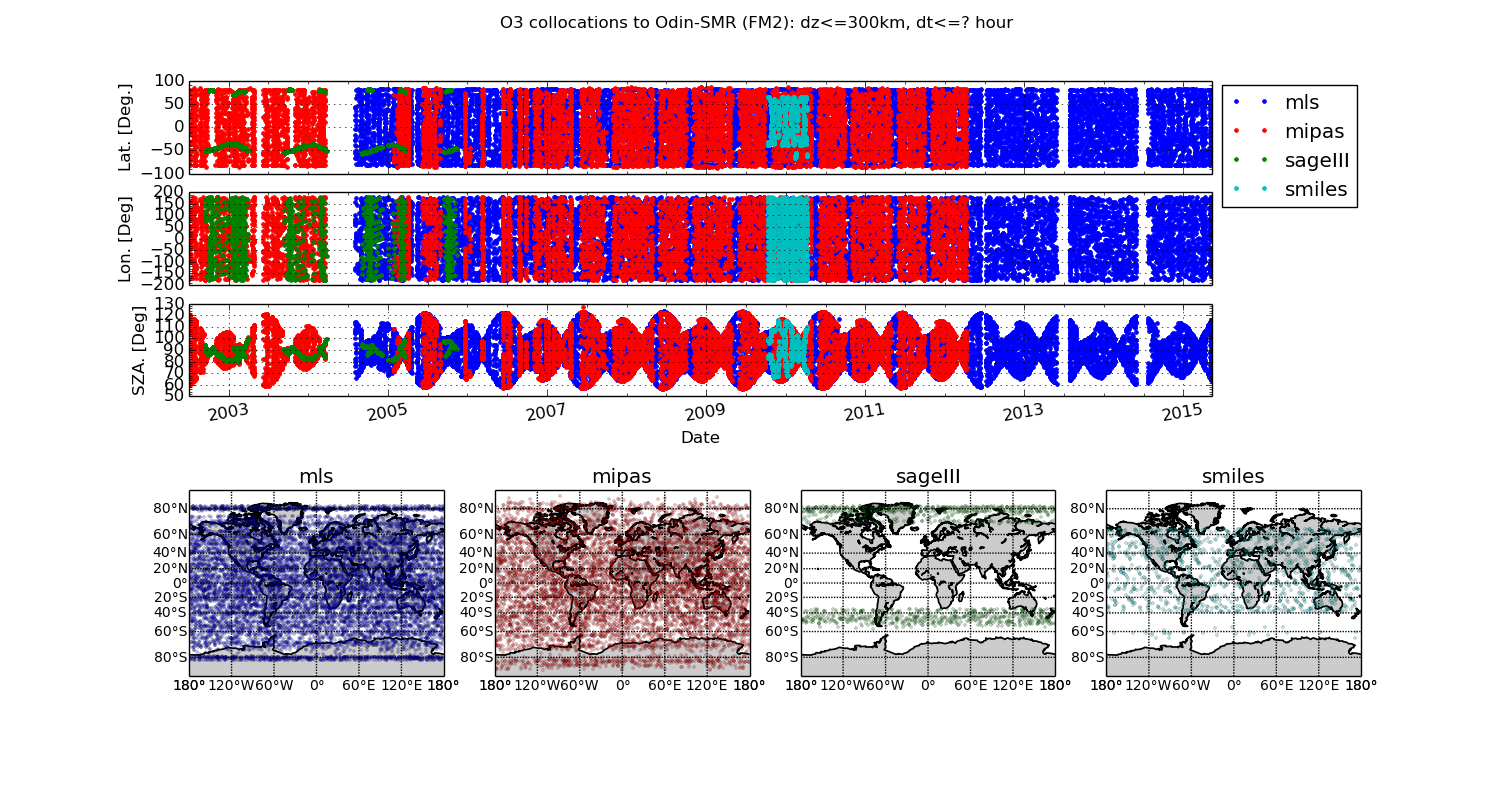
\includegraphics[width=17cm]{test_collocation_fm2.png}
\caption{VDS:Positions of collocated scans for frequency mode 2.}
\label{fig:vdsfm2}
\end{figure}

\clearpage
\newpage

\subsection{Frequency mode 8}

\begin{figure}[t]
\centering
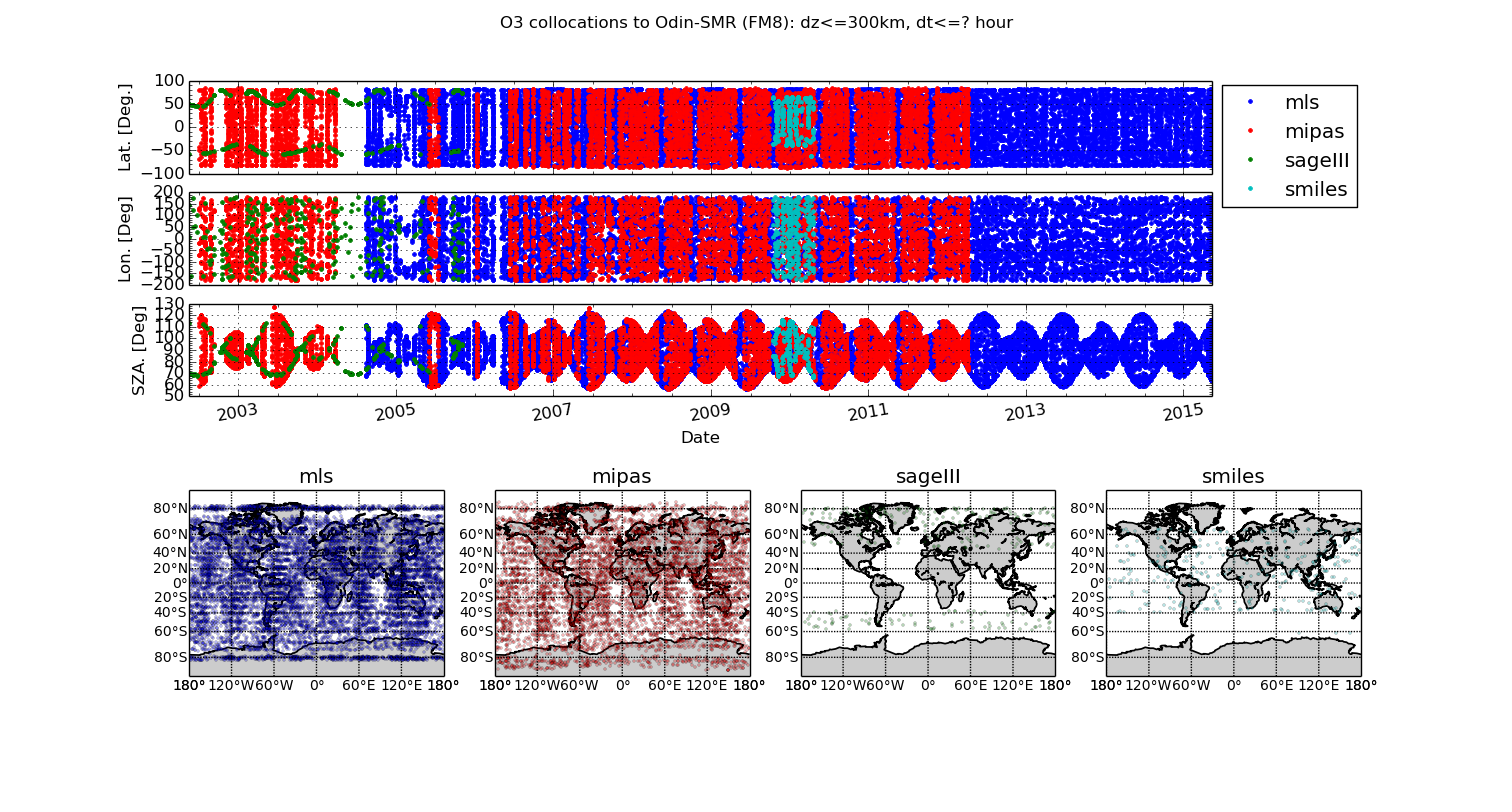
\includegraphics[width=17cm]{test_collocation_fm8.png}
\caption{VDS:Positions of collocated scans for frequency mode 8.}
\label{fig:vdsfm8}
\end{figure}

\clearpage
\newpage

\subsection{Frequency mode 13}

\begin{figure}[t]
\centering
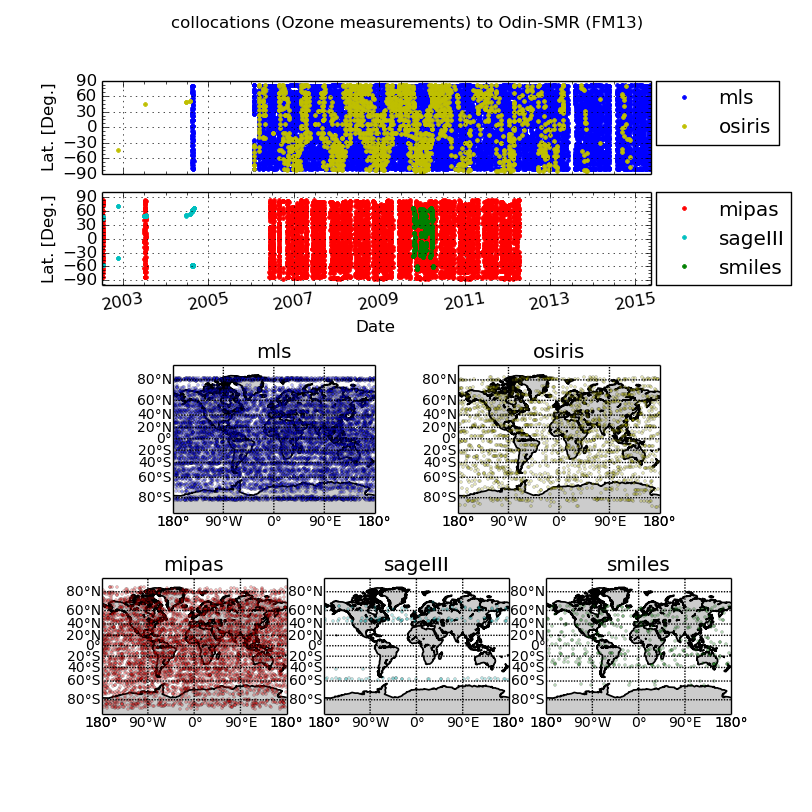
\includegraphics[width=17cm]{test_collocation_fm13.png}
\caption{VDS:Positions of collocated scans for frequency mode 13.}
\label{fig:vdsfm13}
\end{figure}

\clearpage
\newpage

\subsection{Frequency mode 14}

\begin{figure}[t]
\centering
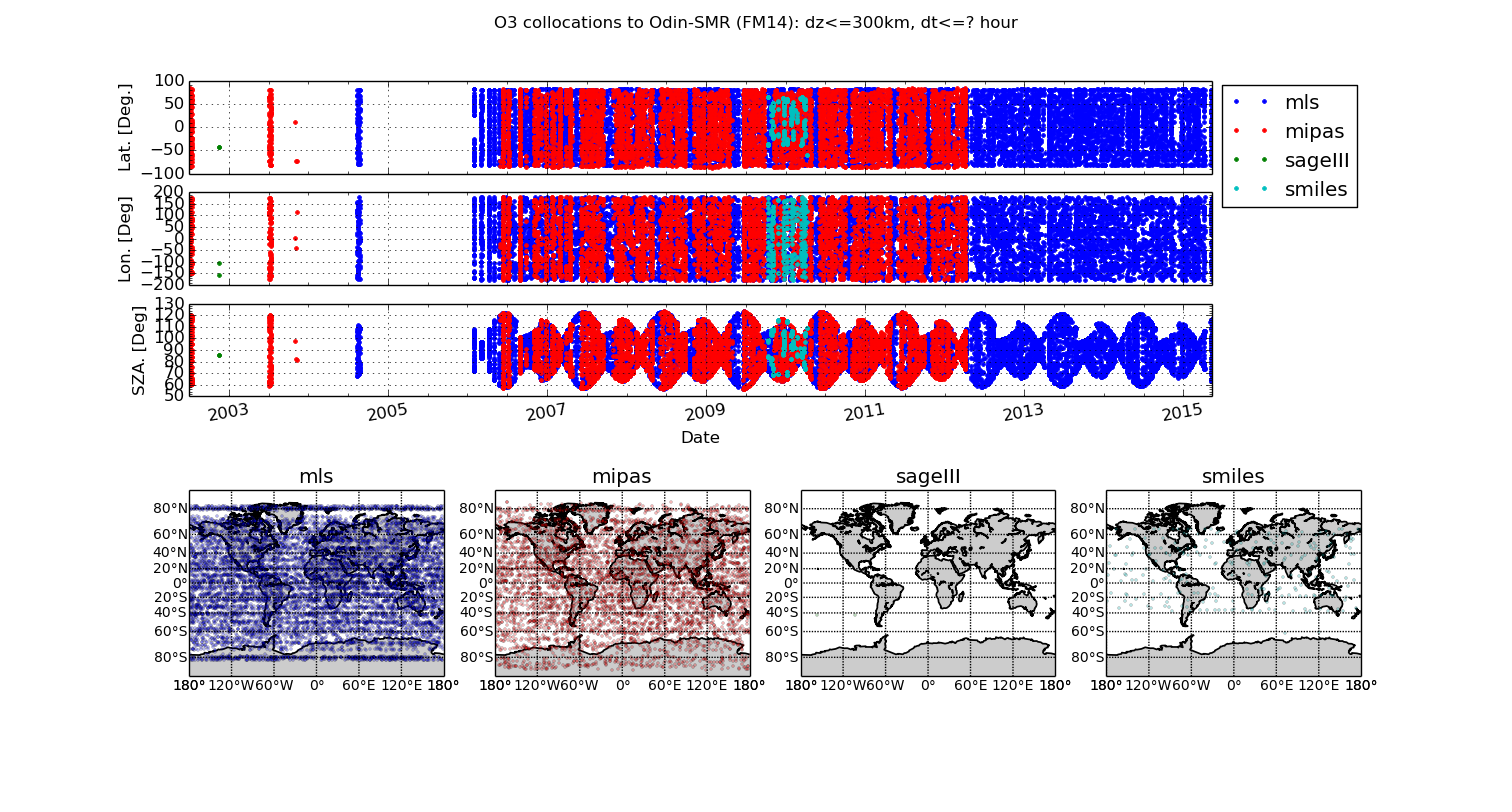
\includegraphics[width=17cm]{test_collocation_fm14.png}
\caption{VDS:Positions of collocated scans for frequency mode 14.}
\label{fig:vdsfm14}
\end{figure}

\clearpage
\newpage

\subsection{Frequency mode 19}

\begin{figure}[t]
\centering
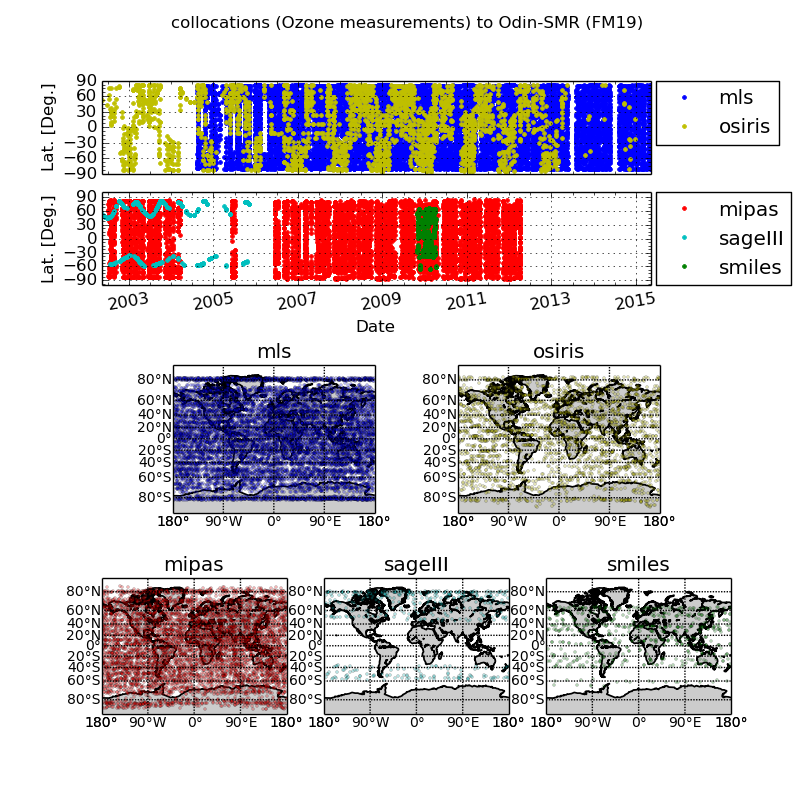
\includegraphics[width=17cm]{test_collocation_fm19.png}
\caption{VDS:Positions of collocated scans for frequency mode 19.}
\label{fig:vdsfm19}
\end{figure}

\clearpage
\newpage

\subsection{Frequency mode 21}

\begin{figure}[t]
\centering
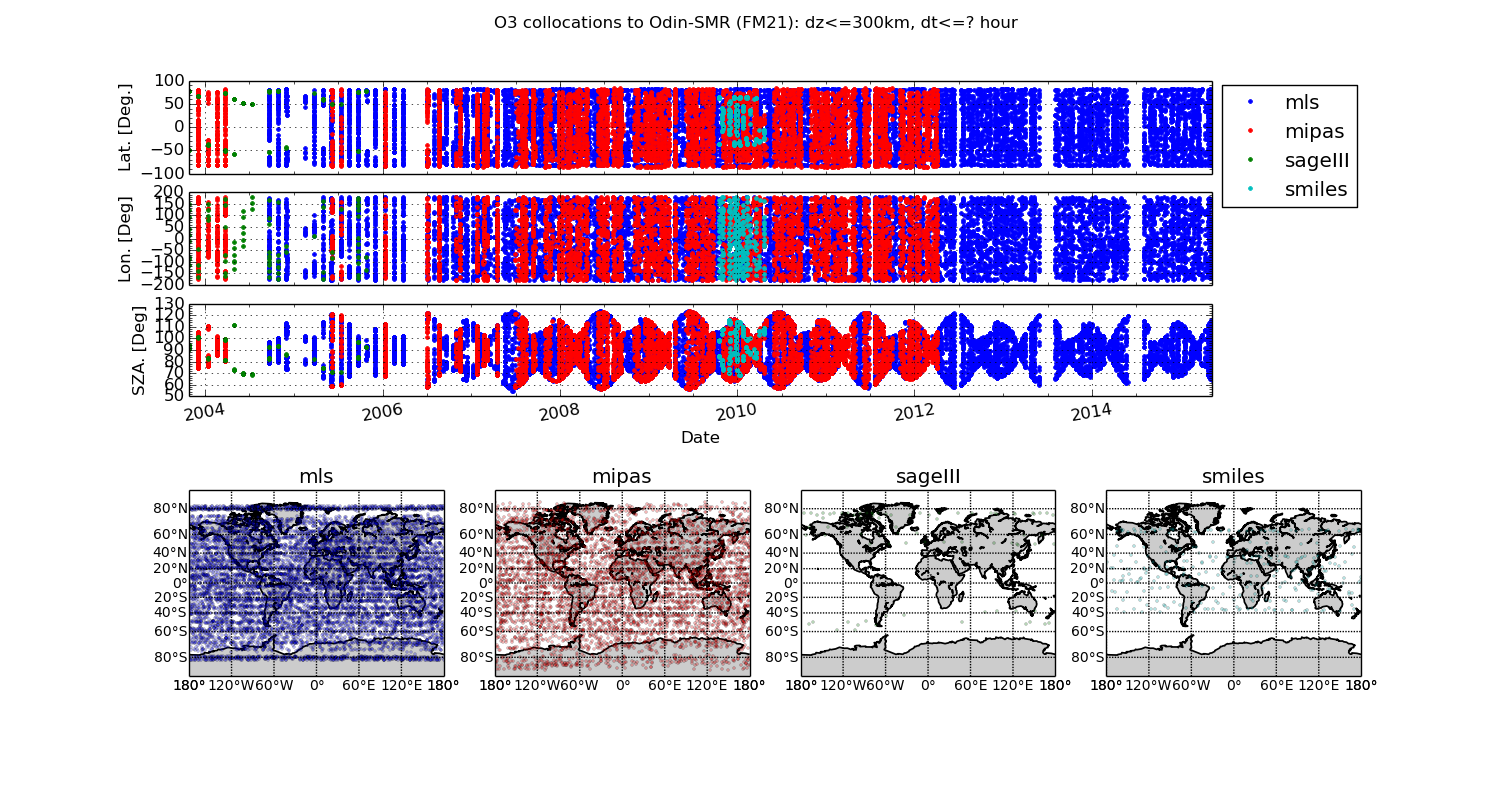
\includegraphics[width=17cm]{test_collocation_fm21.png}
\caption{VDS:Positions of collocated scans for frequency mode 21.}
\label{fig:vdsfm21}
\end{figure}



\section{Data format}
\subsection{Aura/MLS}
...

\subsection{ENVISAT/MIPAS}
...

\subsection{ISS/JEM/SMILES}
...

\subsection{Odin/OSIRIS}
...


\subsection{Meteor3M/SAGE III}
The SAGE III data collocated with Odin/SMR is accessible through the Odin REST
API. The data is returned as a JSON object with the attributes described in
Table~\ref{tab:sage3data}.

\begin{table}
    \caption{Description of attributes in SAGE III JSON object}
    \label{tab:sage3data}
    \begin{tabular}{|l|p{1in}|p{3in}|}
\hline
Attribute & Type & Comment \\
\hline
FileName & String & Filename is the same as in the original data set \\
Instrument & String & Name of the instrument \\
EventType & String & Solar or Lunar (only Solar included in VDS) \\
MJD & List of doubles & Start and end time in MJD for the measurement \\
Latitudes & List of doubles & Start and end latitudes for the measurement \\
Longitudes & List of doubles & Start and end longitudes for the measurement \\
Pressure & List of doubles & Pressure profile for the measurement \\
Temperature & List of doubles & Temperature profile for the measurement \\
<Species> & List of triplets of doubles & Profile for <species> the measurement; each
row contains concentration, uncertainty, and a quality bit
flag\footnote{see \cite{SAGEIII_DPUG} for details!} \\
\hline
    \end{tabular}
\end{table}



